\documentclass[reqno]{amsart}

\usepackage{external/takodachi}
\graphicspath{ {./graphics/} }
\renewcommand{\emph}[1]{\textsc{#1}}

\title
{
	{Ordinary differential equations}
} 

\author{Jason Zhao}
\date{\today}

\begin{document}
\maketitle

\begin{abstract}
	We give an exposition of the initial data problem for ordinary differential equations, with a view towards non-linear evolutionary partial differential equations in mind. The material presented borrows a great deal from \cite[Chapter 1]{Tao2006}. 
\end{abstract}

\tableofcontents

\section{Preliminaries}

\subsubsection*{Geometry of Minkowski space}
Let $(\R^{1 + d}, \bfm)$ denote $(1 + d)$-dimensional Minkowski space with the usual metric, which in rectilinear coordinates $(t, x^1, \dots, x^d)$ takes the diagonal form 
	\[ 
		\bfm = - (\d t)^2 + (\d x^1)^2 + \dots + (\d x^d)^2. 
	\]
We will often write $t = x^0$ for the time coordinate and $x = (x^1, \dots, x^d)$ for the spatial coordinates. We reserve Greek indices, such as $\alpha, \beta, \gamma, \dots$ for space-time coordinates $(t, x^1, \dots, x^d)$, while Latin indices, such as $i, j, k, \ell,\dots$ will be reserved for spatial coordinates $(x^1, \dots, x^d)$. Another useful choice are the polar coordinates $(t, r, \Theta)$ where $r = |x|$ denotes the radius from the origin, and $\Theta := x/|x|$ denotes the radial projection onto the unit sphere $\SS^{d - 1}$. In these coordinates, the Minkowski metric takes the form 
	\[
		\bfm = - \d t^2 + \d r^2 + r^2 g_{\SS^{d - 1}}.
	\]
Denote $\partial_r = \tfrac{x^j}r \partial_j$ the radial vector field and $\nabla_{\SS^{d - 1}}$ for the gradient on the unit sphere $\SS^{d - 1}$. 

\subsubsection*{Geometry of the light cone}

We now introduce notation for the geometry of the light cone and subsets thereof. First and foremost, the forward light cone is defined by 
	\[
		C := \{ (t, x) \in [0, \infty) \times \R^d : r \leq t \}. 
	\]
When studying the light cone, it is convenient to work in null coordinates $(u, v, \Theta)$ defined by $u = t - r$ and $v = t + r$. In these coordinates, the Minkowski metric takes the form 
	\[
		\bfm = - \d u \d v + r^2 g_{\SS^{d -1}}.
	\]
The coordinate vector fields $L = \partial_t + \partial_r = 2 \partial_v$ and $\underline L = \partial_t - \partial_r = 2 \partial_u$ are referred to as null vector fields, as they are parallel to the forward and backwards light cones respectively. Observing that the forward light cone is foliated by surfaces
	\[
		\HH^d_{\rho} := \{ (t, x) \in [0, \infty) \times \R^d : t^2 + r^2 = \rho^2 \},
	\]
we introduce hyperbolic coordinates $(\rho, y, \Theta)$ where $\rho = \sqrt{t^2 - r^2}$ and $y = \tanh^{-1} (r/t)$. Each surface $\HH^d_\rho$ is isometric to the simply connected space of constant sectional curvature $-\tfrac{1}{\rho^2}$. In these coordinates the Minkowski metric takes the form 
	\begin{align*}
		\bfm 
			&= - \d \rho^2 + \rho^2  g_{\HH^d_\rho}\\
			&= - \d \rho^2 + \rho^2 (\d y^2 + \sinh^2 (y) g_{\SS^{d - 1}}).
	\end{align*}
We refer to the vector field $S = \rho \partial_\rho = x^\mu \partial_\mu$ as the scaling vector field, as it is generated from the scaling symmetry of the linear wave equation. 

	\begin{figure}[ht]
		\begin{center}
			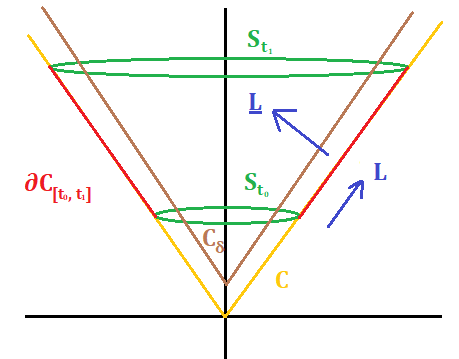
\includegraphics{graphics/cone}
			\caption{The geometry of the light cone. As a wise man once said, a picture is worth $\tfrac1\epsilon$-words for $\epsilon \ll 1$. }
		\end{center}	
	\end{figure}		

\subsubsection*{Subsets of $\R^d$ and $\R^{1 + d}$}
Define the restriction of the light cone to a time interval $I \subseteq [0, \infty)$ and a time slice $t \in [0, \infty)$ respectively by
	\begin{align*}
		C_I 
			&:= C \cap (I \times \R^d), \\
		S_{t}
			&:= C \cap (\{t\} \times \R^d).
	\end{align*}
The \emph{null boundary} $\partial C_I$ denotes the boundary of the time-slab $C_I$ modulo the top and bottom time-slices. Due to singularities on the null boundary, we will also consider the shifted light cone 
	\[ C^\delta := (\delta, 0) + C. \]
Accordingly, we have 
	\begin{align*}
		C^\delta_I
			&:= C_I \cap C^\delta, \\
		S^\delta_t
			&:= S_t \cap C^\delta.		
	\end{align*}	
We also define $B_r (x) \subseteq \R^d$ to be the ball of radius $r$ centered at $x$. 



\section{Existence}
\subsection{Analytic solutions}

Following our earlier remarks, we can formally differentiate the equation to obtain a recurrence relation for the derivatives of $u$. If one specifies initial data at $t = 0$, these relations fully determine all the derivatives $\partial_t^k u (0)$. In the case where the non-linearity is analytic, the formal power series for $u$ is the natural candidate for the solution to the initial data problem. 


\begin{theorem}[Cauchy-Kowalevskaya theorem]
	Let $F \in C^\omega (\R^n \to \R^n)$ be analytic, then there exists a unique analytic solution to the initial data problem (\ref{eq:idp}). 
\end{theorem}

\begin{proof}
	By replacing $u$ with $u - u_0$, it is not a loss of generality to prove solve the equation for initial data $u_0 = 0$. Our goal is to obtain an \textit{a priori} estimate on the growth of $\partial_t^m u(0)$ such that the \textit{ansatz}
		\[ u(t) := \sum_{n = 0}^\infty \frac{\partial^n_t u (0)}{m!} t^m \]	
	is shown to be analytic. It would follow by construction and the uniqueness theorem then that $\partial_t u - F(u) \equiv 0$ since the left-hand side is an analytic function which vanishes to every order at $t = 0$. Formally differentiating the equation, it follows from the chain rule and induction that the derivatives of $u$ can be written as a polynomial with non-negative coefficients in the derivatives of $F$ up to order $m - 1$,
		\[ \partial_t^m u = p_m ( F (u),  \nabla F(u), \dots, \nabla^{m - 1} F(u)) \]
	for some $p_m \in \N_0 [\vec x]$. Using the initial data $u(0) = 0$, it follows that $\partial_t^m u (0)$ are fully determined by $\nabla^j F(0)$ up to order $j < m$. Note that the polynomial $p_m$ is determined combinatorially, depending only on the order $m$. To estimate the growth of $\partial_t^m u (0)$, we argue by \textit{analytic majorisation}; non-negativity of the coefficients of $p_m$ imply 
		\begin{equation}
			|\partial^m_t u (0)| \leq \partial^m_t v(0)
			\tag{*}
			\label{eq:major}  
		\end{equation}	
	for any solution to the initial data problem	
		\begin{align*}
			\partial_t v 
				&= G(v) ,\\
			v_{|t = 0}
				&= 0,	
		\end{align*}
	for some analytic $G \in C^\omega (\R^n \to \R^n)$ such that $|\partial^m F_i (0)| \leq \partial^m G_i (0)$. Our strategy will be to choose $G$ such that the auxiliary ODE above is explicitly solvable for analytic $v$. The growth estimates on the power series of coefficients of $v$ also hold for those of $u$ via the majoristion (\ref{eq:major}), completing the proof. To construct $G$, we know from analyticity of $F$ that there exists $r > 0$ such that
		\[ |\nabla^m F(0)| \leq \frac{m!}{r^{m + 1}}. \]
	We construct $G$ such that the $m$-th order derivatives are precisely the right-hand side, namely
		\[  G_i (z_1, \dots, z_n) := \frac{1}{r - z_1 - \dots - z_n}. \]	
	For simplicity, consider the scalar case $n = 1$, the higher dimensional case is similar. By separation of variables, the explicit solution is given by $v(t) = r - r \sqrt{1 - 2t}$, which is clearly analytic in the region $|t| < r/2$. This completes the proof. 
\end{proof}


\subsection{Picard iteration}

	From the strong solution perspective, solving (\ref{eq:idp}) is equivalent to finding a \emph{fixed point} $\Phi_{u_0} (u) = u$ of the integral operator $\Phi_{u_0} : C^0 ([0, T] \to \R^n) \to C^0 ([0, T] \to \R^n)$ defined by 
		\[ (\Phi_{u_0} u)(t) := u_0 + \int_0^t F(u(s)) \, ds. \]
	We will argue by \textit{Picard iteration}. Schematically, we start off with an approximate solution $u_0$, and inductively construct subsequent approximates $u_{n}$ by inputting $u_{n - 1}$ into the integral operator,
		\[ u_n := \Phi_{u_0} (u_{n - 1}) = u_0 + \int_0^t F(u_{n - 1}(s)) \, ds .\]
	These approximate solutions are known as \emph{Picard iterates}, and the goal then is to show that this sequence $\{u_n\}_n$ converges uniformly to some $u$. If this were true, then by continuity of $\Phi_{u_0}$ and construction of the sequence, the limit $u$ would be a fixed point. A sufficient condition is if $\Phi_{u_0}$ is a \emph{contraction}, i.e. Lipschitz continuous with constant $L < 1$, 
	\[ || \Phi_{u_0} (u) - \Phi_{u_0} v||_{C^0[0, T]} \leq L ||u - v||_{C^0[0, T]}. \]
	\begin{figure}[h]
		\begin{center}
			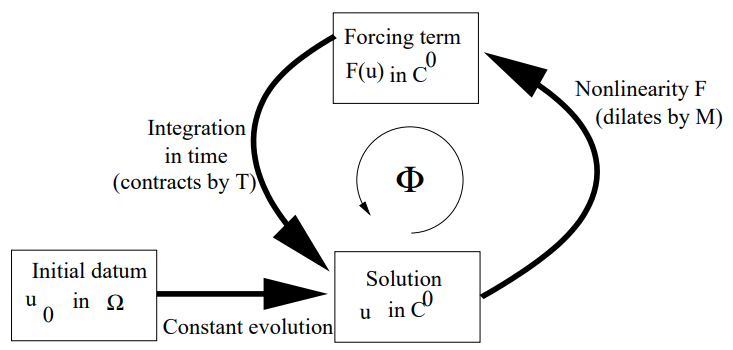
\includegraphics[scale = 0.6]{picard}
			\caption{The strong solution notion says that $u$ is determined by its past via integration in time. Thus for $T \ll 1$, the initial data $u_0$ is a good approximate solution. Iterating these approximations through the operator $\Phi_{u_0}$ converges provided we have some ``gain'' at each stage. }
		\end{center}
	\end{figure}
	
\begin{lemma}[Contraction mapping principle]
	Let $(X, d)$ be a complete non-empty metric space, and let $\Phi : X \to X$ be a contraction on $X$. Then there exists a unique fixed point $u = \Phi(u)$. Furthermore, if $u_0 \in X$ and we construct the sequence $\{u_n\}_n \subseteq X$ iteratively by 
		\[ u_{n + 1} := \Phi(u_n),\]
	then $u_n \to u$. 
\end{lemma}

\begin{proof}
	To show existence, we aim to show that the iterates $\{u_n\}_n$ form a Cauchy sequence. For $n, k \geq 0$, we obtain
		\begin{alignat*}{2}
			 d(u_n, u_{n + k}) 
			 	&= d(\Phi^n (u_0), \Phi^n (u_k))			
			 		&&\\
			 	&\leq c^n d(u_0, u_k) 
			 		&&\\
			 	&\leq c^n \left( d(u_0, \Phi(u_0)) + \dots + d(\Phi^{k - 1} (u_0), \Phi^k (u_0)) \right) 
			 		&&, \\
			 	&\leq 	c^n \sum_{j = 0}^{k - 1} c^j d(u_0, \Phi(u_0))
			 		&& \\
			 	&\leq \frac{c^n}{1 - c} d(u_0, \Phi(u_0))
			 		&&.	
		\end{alignat*}	 
	Since $0 < c < 1$, the above vanishes upon passing the limit $n \to \infty$, proving that the sequence is Cauchy. Since $X$ is complete, we know that there exists a limit $u \in X$. As contractions are continuous, 
		\[ \Phi(u) = \Phi( \lim_{n \to \infty} u_n) = \lim_{n \to \infty} \Phi(u_n) = \lim_{n \to \infty} u_{n + 1} = u.  \]
	To show uniqueness, suppose $v \in X$ is another fixed point, then by definition and the contraction inequality
		\[ d(u, v) \leq cd(u, v), \]	
	which, since $0 < c < 1$, can only hold if $d(u, v) = 0$ i.e. $u = v$. 
\end{proof}

\begin{theorem}[Picard-Lindelof existence theorem]
	Let $\Omega \subseteq \R^d$ be a domain, and suppose $F \in \dot C^{0, 1}_{\loc} (\Omega \to \R^d)$ is locally Lipschitz. For initial data $u_0 \in \Omega$ and $\epsilon \ll 1$, set
		\begin{align*}
			L
				&:= ||F||_{\dot C^{0, 1} (\overline{B_\epsilon (u_0)})} ,\\
			M
				&:= ||F||_{C^{0} (\overline{B_\epsilon (u_0)})}.	
		\end{align*}
	Then for $T < \min (\epsilon/M, 1/L)$, there exists a strong solution $u: [0, T] \to \overline{B_\epsilon (u_0)}$ to the initial data problem (\ref{eq:idp}). 
\end{theorem}

\begin{proof}
	The contraction mapping principle furnishes a solution provided we show that the integral operator $\Phi_{u_0}$ is a contraction mapping on the closed ball $C^0 ([0, T] \to \overline{B_\epsilon (u_0)})$. We first show $\Phi_{u_0}$ maps the desired space into itself: by choice of $T$ and $M$, we have 
		\begin{align*}
			 ||(\Phi_{u_0} u)(t) - u_0||_{C^0 [0, T]} 
			 	&\leq \int_0^T |F(u(s))| \, ds \leq TM \leq \epsilon. 
		\end{align*}
	Next, we show $\Phi_{u_0}$ is a contraction: 
		\[ ||\Phi_{u_0} u - \Phi_{u_0} v||_{C^0 [0, T]} \leq  \int_0^T |F(u(s)) - F(v(s))| \, ds \leq T L ||u - v||_{C^0}, \]
	where $TL < 1$ by construction. This completes the proof.
\end{proof}

\begin{remark}
	A common theme in solving ODEs and more generally PDEs is that we need to exploit some ``smallness'' to get an estimate or iteration to close. In this case, we exploit the time of existence $T$ to ``defeat'' any large oscillations from $F$ which could prevent the iteration from converging. 
\end{remark}


\subsection{Compactness solutions}

Suppose now we only had continuity of the non-linearity $F$ and no control over the Lipschitz norms. We again argue by approximation, this time approximating the equation and showing the corresponding solutions converge via \textit{compactness}, namely 

\begin{lemma}[Arzela-Ascoli theorem]
	Let $(X, d)$ be a compact metric space, and let $\cF \subseteq C(X)$ be a family of continuous functions. Then $\cF$ is pre-compact if and only if 
	\begin{itemize}
		\item $\cF$ is uniformly bounded, that is, $||f||_{C(X)} \lesssim 1$ uniformly in $f \in \cF$, 
		\item $\cF$ is equicontinuous, that is, for every $\epsilon > 0$ there exists a uniform $\delta > 0$ such that $|f(x) - f(y)| < \epsilon$ whenever $|x - y| < \delta$ for all $f \in \cF$.
	\end{itemize}
\end{lemma}

While we can approximate the non-linearity in the uniform topology by Lipschitz functions, there is no uniform control over the Lipschitz constants. Thus, following the proof of the Picard-Lindelof theorem, we cannot quantitatively show the approximate solutions exist on the same time interval existence. We instead turn to a more qualitative argument relying on \textit{continuous induction on time}. 

\begin{lemma}[Bootstrap argument]
	Let $f : [0, T) \to [0, \infty)$ be continuous, and suppose $f(0) \leq C$. Suppose that $f(t) \leq 2C$ implies the stronger bound $f(t) \leq C$, then the stronger bound holds for all time. 
\end{lemma}

\begin{proof}
	We argue by connectedness of the interval $[0, T)$. The set of times $A \subseteq [0, T)$ where $f(t) \leq 2C$ holds is
		\begin{itemize}
			\item non-empty, since $0 \in A$, 
			\item closed, since $f$ is continuous, 
			\item open, since if $t \in A$, then we in fact have the stronger bound $f(t) \leq C$, which by continuity allows us to propagate the weaker bound forward in time $f(t^+) \leq 2C$. 
		\end{itemize}
	Hence $A = [0, T)$. 
\end{proof}

\begin{remark}
	The weaker estimate $f(t) \leq 2C$ is known as a \emph{bootstrap assumption}. Since it in fact implies a stronger bound $f(t) \leq C$, the estimate ``picks itself up by its bootstraps''. 
\end{remark}

\begin{theorem}[Peano's existence theorem]
	Let $\Omega \subseteq \R^n$ be a domain and suppose $F \in C^0_{\loc} (\Omega \to \R^n)$ is continuous. Then for any $u_0 \in \Omega$, there exists a local solution to the initial data problem (\ref{eq:idp}).
\end{theorem}

\begin{proof}
	Assume without loss of generality $u_0 = 0$. There exists $\{ F_k \}_k \subseteq C^\infty (\Omega \to \R^n)$ such that $F_k \to F$ uniformly on compact sets. Smooth functions are locally Lipschitz, so, choosing a small closed ball $\overline{B_\epsilon (0)} \subseteq \Omega$, Picard-Lindelof furnishes local solutions $u_k : [0, T_k) \to B_\epsilon (0)$ to the initial data problems
	\begin{align*}
		\partial_t u_k 	
			&= F_k(u_k), \\
		{u_k}_{|t = 0}		
			&= 0
	\end{align*}
	We claim that there exists a uniform time interval $[0, T] \subseteq \bigcap_k [0, T_k)$ on which $\{u_k\}_k$ exist and are pre-compact. By uniform convergence, there exist uniform constant $M > 0$ such that $|F_k (u)| \leq M$ whenever $|u| \leq \epsilon$. Let $0 < T < \epsilon/(2M + 1)$, we make the bootstrap assumption that $|u_k| \leq \epsilon$ on the interval $[0, T]$. It follows that
		\[ |u_k (t)| \leq \int_0^T |F_k (u_k (s))| \, ds \leq T M \leq \frac\epsilon2 \]
	for all $t \in [0, T]$. The local well-posedness theory allows us to continue the solution, thus by continuous induction on time $u_k$ exists on $[0, \epsilon/(2M + 1)$ and satisfies the uniform bound $|u_k| \leq \epsilon$. Furthermore the equation implies $|\partial_t u_k| \leq M$. This proves $\{u_k\}_k$ is uniformly bounded and equicontinuous, so by Arzela-Ascoli we pass to a subsequence which converges uniformly to a continuous function $u$. As $F_k (u_k (t)) \to F(u(t))$ uniformly, we conclude $u$ is a desired strong solution, i.e. 
		\[ u(t) = \lim_{k \to \infty} u_k (t) = \lim_{k \to \infty} \int_0^t F_k (u_k (s)) \, ds = \int_0^t F (u(s)) \, ds\]
	for all $t \in [0, \epsilon/(2M + 1)]$. 	
\end{proof}


\begin{remark}
	Uniqueness may fail without further assumptions on the regularity of $F$; for example, letting $0 < \alpha < 1$, consider the initial data problem
			\begin{align*}
				\partial_t u 	&= |u|^\alpha, \\
				u_{|t = 0}		&= 0.
			\end{align*}
	Then 
		\[
			u_c (t) = 
				\begin{cases}
					0, 												&\text{if } x \leq c, \\
					(t - c)^\frac{1}{1 - \alpha}, 	&\text{if } t > c,
				\end{cases}
		\]		
	is an infinite family of solutions indexed by $c \geq 0$. Following the proof of Peano's existence theorem, we observe that uniqueness breaks down in that our solution depends on the choice of approximation by smooth functions. 
	
	\begin{figure}[h]
	\begin{center}
		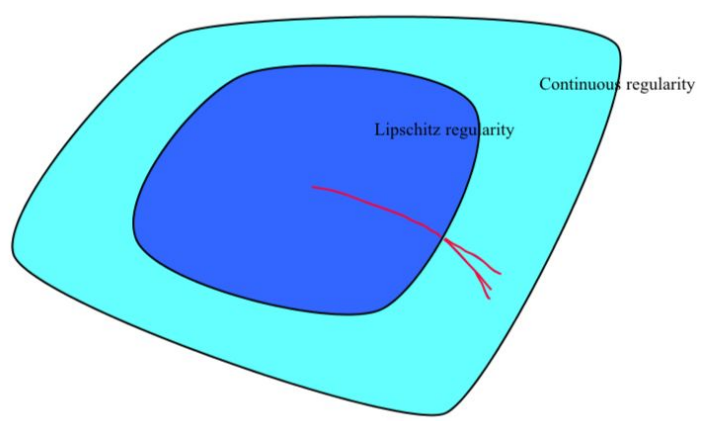
\includegraphics[scale = 0.5]{unique}
		\caption{Uniqueness fails once the solution leaves the regime of Lipschitz regularity. Approaching the boundary can be viewed as a \textit{blow-up criterion}, see Section 5 for details. }
	\end{center}
\end{figure}
\end{remark}

\section{Uniqueness}
As seen in Peano's theorem, uniqueness breaks down once the solution leaves the regime where the non-linearity is Lipschitz continuous. Thus we restrict our attention to solutions which stay within the state space $\Omega$. In this regime, we have uniqueness for $F \in \dot C^{0, 1}_{\loc} (\Omega \to \R^n)$, complementing the local existence theory. Our key ingredient will be Gronwall's inequality, which states that linear feedback bounds can at worst lead to exponential growth. 

\begin{lemma}[Gronwall's integral inequality]
	Let $u: [0, T] \to \R^+$ be a continuous and non-negative function, and suppose $u$ obeys the integral inequality
		\[ u(t) \leq A + \int_0^t B(s) u(s) \, ds \]
	for some $A \geq 0$ and $B :[0, T] \to \R^+$ continuous and non-negative. Then 
		\[ u(t) \leq A \exp \left( \int_0^t B(s) \,ds \right). \]	
	Moreover, this estimate is sharp, with equality when $u(t) := A \exp (\int_0^t B(s) \, ds)$. 	
\end{lemma}

\begin{proof}
	By a limiting argument we can assume $A > 0$. Differentiating the right-hand side of the integral inequality, the fundamental theorem of calculus and the inequality imply
		\[ \frac{d}{dt} \left(A + \int_0^t B(s) u(s) \, ds \right) \leq B(t) \left( A + \int_0^t B(s) u(s) \, ds \right) .\]
	Hence by the chain rule
		\[ \frac{d}{dt} \log \left(  A + \int_0^t B(s) u(s) \, ds  \right) \leq B(t). \]	
	Integrating, we obtain
		\[  \log \left(  A + \int_0^t B(s) u(s) \, ds  \right) \leq \log A + \int_0^t B(s) \, ds, \]
	which upon exponentiating completes the proof. 		
\end{proof}

\begin{theorem}[Picard-Lindelof uniqueness theorem]
	Let $\Omega \subseteq \R^n$ be a domain, and suppose $F \in \dot C^{0, 1}_{\loc} (\Omega \to \R^n)$ is locally Lipschitz. If $u, v \in C^1_{\loc} ([0, T] \to \Omega)$ are solutions to the initial data problem (\ref{eq:idp}), then $u \equiv v$. 
\end{theorem}

\begin{proof}
	Since $[0, T]$ is a compact interval, $u$ and $v$ range over a compact subset of $\Omega$. Therefore by local Lipschitz continuity there exists $L > 0$ such that $|F(u) - F(v)| \leq L |u - v|$. The difference of the two solutions satisfy
		\[ \partial_t (u - v) = F(u) - F(v).\]
	Integrating and applying the triangle inequality gives 
		\[ |u(t) - v(t)| \leq \int_0^t |F(u(s)) - F(v(s))| \, ds \leq L \int_0^t |u(s) - v(s)| \, ds .\]
	We conclude from Gronwall's inequality that $u \equiv v$. 	
\end{proof}

\section{Continuous dependence on initial data}
Studying the proof of the Picard-Lindelof existence theorem, we see that the corresponding solutions to initial data in any domain $\Omega \subseteq \R^n$ can be taken to exist on the same time-interval $[0, T]$, provided there exists a uniform bound and Lipschitz constant on an $\epsilon$-neighborhood $\overline{B_\epsilon (\Omega)} \subseteq \R^n$. Combined with uniqueness, the \emph{solution operator} $S : \Omega \to C^0 ([0, T] \to \R^n)$ mapping initial data to solutions is well-defined. Our goal in this section will be to study the regularity of this operator. 



\subsection{$C^{0, 1}$-dependence}

We begin with Lipschitz dependence on initial data. This is a simple consequence of retracing the proof of the Picard-Lindelof theorem and tracking down the constants. 

\begin{theorem}[$C^{0, 1}$-dependence on data]
	Let $\Omega \subseteq \R^n$ be a domain, and suppose $F \in C^{0, 1}(\overline{B_\epsilon (\Omega)} \to \R^n)$ is Lipschitz and bounded with constants
		\begin{align*}
			L &:= ||F||_{\dot C^{0, 1} (\overline{B_\epsilon (\Omega)})}, \\
			M &:= ||F||_{C^{0} (\overline{B_\epsilon (\Omega)})}.
		\end{align*}
	Then for $T< \min (\epsilon/M, 1/L)$, the solution operator $S : \Omega \to C^0 ([0, T] \to \R^n)$	 is well-defined and Lipschitz continuous with constant $\frac{1}{1 - TL}$.
\end{theorem}

\begin{proof}
	The solution $S u_0$ is a fixed point of $\Phi_{u_0}$, so we can write
		\[ S u_0 - Sv_0 = \Phi_{u_0} (S u_0) - \Phi_{v_0} (S v_0) + u_0 - v_0. \]
	Following the Picard-Lindelof existence proof, we showed that the integral operators $\Phi_{u_0}$ are contractions on $C^0([0, T] \to \Omega)$ for every initial data $u_0 \in \Omega$ with Lipschitz constant $TL$. Thus, taking norms above and applying the triangle inequality, we obtain 
		\[ || Su_0 - Sv_0||_{C^0 [0, T]} \leq ||\Phi_{u_0} (Su_0) - \Phi(S v_0)||_{C^0 [0, T]} + |u_0 - v_0| \leq  TL || Su_0 - Sv_0||_{C^0 [0, T]} + |u_0 - v_0|.\]
	Rearranging, 
		\[ || Su_0 - Sv_0||_{C^0 [0, T]} \leq \frac{1}{1 - TL} |u_0 - v_0|,  \]
	as desired. 		
\end{proof}

\subsection{$C^1$-dependence}

Assume the non-linearity is continuously differentiable, we want to show that the solution operator is continuously differentiable. This is meant in the \textit{Frechet} sense, i.e. there exists a linear operator $DS(u_0) : \R^n \to C^0 ([0, T] \to \R^n)$ such that 
	\[ \lim_{v \to 0}\left|\left| \frac{S(u_0 + v) - S(u_0) - DS(u_0)}{|v|} \right|\right|_{C^0[0, T]} = 0 \]
and $u_0 \to DS(u_0)$ is continuous. As in the finite-dimensional codomain setting, this is equivalent to the existence and continuity of ``partial'' Frechet derivatives, so we will consider smooth one-parameter families of initial data $h \mapsto u_0 (h)$ for $|h| \ll 1$, and show that the solution $u(t, h) := Su_0 (h) (t)$ is continuously differentiable in $h$. The total derivative $DS$ can be reconstructed from the partial derivatives $\partial_h u$.

 The difference quotient in $h$ satisfies 
	\[ \partial_t \left( \frac{u(t, h) - u(t, 0)}{h} \right) = \frac{F(u(t, h)) - F(u (t, h_0))}{h},  \]
then, assuming $u$ is continuously differentiable in $h$ and $F$ is continuously differentiable, taking $h \to 0$ gives
	\[ \partial_t \partial_h u (t, 0) = \nabla F(u(t, 0)) \cdot \partial_h u (t, 0). \]
This shows that $\partial_h u$, if it exists, satisfies the \emph{linearised equation},
	\begin{equation}
		\begin{split}
			\partial_t A 
		 	&= \nabla F (u) \cdot A,\\
		 A_{|t = 0}
		 	&= \partial_h u_0 (0)	.
		\end{split}
		\tag{Lin}
		\label{eq:linear}
		\end{equation}
\textit{A priori}, we do not know if $u$ is continuously differentiable with respect to its initial data, so we instead work backwards by studying the linearised initial data problem. Heuristically, the \textit{dynamics} of the original equation are dominated by the linearised equation, as the higher-order terms in the non-linearity are negligible. 


\begin{theorem}[$C^{1}$-dependence on data]
	Let $\Omega \subseteq \R^n$ be a domain, and suppose $F \in C^{1}(\overline{B_\epsilon (\Omega)} \to \R^n)$ is continuously differentiable and bounded with constants
		\begin{align*}
			L &:= ||F||_{\dot C^{1} (\overline{B_\epsilon (\Omega)})}, \\
			M &:= ||F||_{C^{0} (\overline{B_\epsilon (\Omega)})}.
		\end{align*}
	Then for $T< \min (\epsilon/M, 1/L)$, there exists a unique solution $u \in C^2_{\loc} ([0, T] \to \R^n)$ to (\ref{eq:idp}), and the solution operator $S : \Omega \to C^0 ([0, T] \to \R^n)$	 is well-defined and continuously differentiable.
\end{theorem}

\begin{proof}
	Using the equation and the chain rule, we see that the solution obtained from Picard-Lindelof iteration has regularity $u \in C^2_{\loc} ([0, T] \to \R^n)$. By local well-posedness, the linearised equation (\ref{eq:linear}) admits a solution in $[0, T]$. We claim that $\partial_h u(t, 0)$ exists and $A = \partial_h u (t, 0)$. Translating, this argument shows that $\partial_h u (t, h)$ exists for all $t \in [0, T]$ and $|h| \ll 1$. Set
		\[ B(t) := \frac{u(t, h) - u(t, 0)}{h} - A(t) , \]
	our goal is to show that $B (t) \to 0$ as $h \to 0$ for each fixed $t$. Differentiating and using the equations, 
		\begin{align*}
			\partial_t B (t)
				&= \frac{F(u(t, h)) - F(u(t, 0))}{h} - \nabla F(u(t, 0)) \cdot A(t)  \\
				&=  \int_0^1 \frac{u(t, h) - u(t, 0)}{h} \cdot \nabla F(s \cdot u(t, h) + (1 - s) \cdot u (t, 0)) \, ds - \nabla F(u(t, 0)) \cdot A(t) \\
				&= C_1 (t) \cdot B(t) + C_2 (t) \cdot A(t),
		\end{align*}	
	where
		\begin{align*}
			C_1 (t) 
				&:=\int_0^1 \nabla F(s \cdot u(t, h) + (1 - s) \cdot u (t, 0)) \, ds, \\
			C_2 (t)
				&:= \int_0^1  \left(\nabla F(s\cdot u(t, h) + (1 - s)\cdot u (t, 0)) - \nabla F (u(t, 0))\right)\, ds .
		\end{align*}	
	From our regularity assumptions, we see that $|A|, |C_1|, |C_2| \leq N$ for some uniform constant $N \gg 1$. Thus, integrating the expression for $\partial_t B$ and applying the bounds above, we obtain 
		\[ |B(t)| \leq |B(0)| + TN ||C_2||_{C^0[0, T]}  + N \int_0^t |B(s)| \, ds.  \]	
	Using Gronwall's inequality, this implies
		\[ |B(t)| \leq e^{t} \left( |B(0)| + TN ||C_2||_{C^0[0, T]} \right)  \]	
	Since $h \mapsto u(0, h)$ and $F$ are continuously differentiable, $|B(0)|$ and $||C_2||_{C^0[0, T]}$ vanish as $h \to 0$. We conclude from construction of $B$ that $\partial_h u$ exists and is given by $A$. 
	
	It remains to show that $\partial_h u$ is continuous in $h$ uniformly in $t$. Again, by translation it is not a loss of generality to show the result for $h = 0$. Integrating the linearised equation, we obtain
		\begin{align*}
			|\partial_h u (t, h) - \partial_h u (t, 0)|
				&\leq |\partial_h u(0, h) - \partial_h u (0, 0)| + \int_0^t |\nabla F (u(s, h)) \cdot \partial_h u (s, h) - \nabla F(u(s, 0)) \cdot \partial_h u(s, 0)| \, ds\\
				&\leq |\partial_h u(0, h) - \partial_h u (0, 0)| + \int_0^t |\nabla F (u(s, h)) - \nabla F(u(s, 0))|  \cdot |\partial_h u(s, h)| \, ds \\
				&\qquad+ \int_0^t |\nabla F(u(s, 0)) \cdot | \partial_h u(s, h) - \partial_h u(s, 0)| \, ds
		\end{align*}
	By Gronwall's inequality.
		\[ |\partial_h u (t, h) - \partial_h u (t, 0)| \leq e^{L t} \left( |\partial_h u_0 (h) - \partial_h u_0 (0)| + C \int_0^t   |\nabla F (u(s, h)) - \nabla F(u(s, 0))| \, ds \right) \]	
	for some $L, C > 0$. Since $\partial_h u_0$ and $\nabla F$ are continuous, the right-hand side vanishes uniformly in $t$ as $h \to 0$. 	
\end{proof}

\begin{corollary}[$C^{k}$-dependence on data]
	Let $\Omega \subseteq \R^n$ be a domain, and suppose $F \in C^{k}(\overline{B_\epsilon (\Omega)} \to \R^n)$ is continuously differentiable and bounded with constants
		\begin{align*}
			L &:= ||F||_{C^{k} (\overline{B_\epsilon (\Omega)})}, \\
			M &:= ||F||_{C^{0} (\overline{B_\epsilon (\Omega)})}.
		\end{align*}
	Then for $T< \min (\epsilon/M, 1/L)$, the solution operator $S : \Omega \to C^0 ([0, T] \to \R^n)$	 is well-defined and continuously differentiable.
\end{corollary}

\begin{proof}
	Induction on $k$ and the $C^1$-wellposedness theory. 
\end{proof}

\section{Maximal solutions}
In the previous sections, we have studied the \textit{local} well-posedness theory of the initial data problem. Inductively applying the local theory to the end-time of existence for any solution $u$, we can show that there exists a \emph{maximal time of existence} $T_{\text{max}}$, i.e. there does not exist a solution $v : [0, T^+] \to \R^n$ to (\ref{eq:idp}) such that $u \equiv v$ on $[0, T_{\text{max}})$. We refer to the solution defined on $[0, T_{\text{max}})$ as the \emph{maximal solution}. 

\begin{theorem}[Continuation criterion]
	Let $\Omega \subseteq \R^n$ be a domain, and suppose $F \in \dot C^{0, 1}_{\loc} (\Omega \to \R^n)$ is locally Lipschitz. If $u : [0, T] \to \Omega$ is a solution to the initial data problem (\ref{eq:idp}) which does not approach the boundary of $\Omega$ or blow-up, i.e.
		\begin{align*}
			\lim_{t \to T}\operatorname{dist} (u(t), \partial \Omega) 
				> 0, \qquad \text{and} \qquad
			\lim_{t \to T} |u(t)| 
				< \infty,
		\end{align*}
	then $u$ can be extended to a solution on $[0, T^+]$. 
\end{theorem}

\begin{proof}
	Since $u$ does not approach the boundary or blow-up, there exists a closed ball $\overline{B_\epsilon(u(T))} \subseteq \Omega$ on which we can continue the solution via the local theory. 
\end{proof}

\begin{corollary}[Existence of maximal solutions]
	Let $\Omega \subseteq \R^n$ be a domain, and suppose $F \in \dot C^{0, 1}_{\loc} (\Omega \to \R^n)$ is locally Lipschitz. Then there exists a maximal solution defined on a half-open interval $[0, T_{\text{max}})$. 
\end{corollary}

\begin{proof}
	The maximal time interval of existence must be half-open, since if $u$ is defined on $[0, T]$, then by local well-posedness it can be extended to $[0, T^+]$. Define the maximal time interval of existence $[0, T_{\text{max}})$ as the union of all intervals $[0, T]$ for which one has a solution to the initial data problem (\ref{eq:idp}). By the uniqueness theorem, we may glue these solutions together to obtain a maximal solution.
\end{proof}

\begin{corollary}[Blow-up criterion]
	Let $\Omega \subseteq \R^n$ be a domain, and suppose $F \in \dot C^{0, 1}_{\loc} (\Omega \to \R^n)$ is locally Lipschitz. If $u$ is a maximal solution to the initial data problem (\ref{eq:idp}) and $T_{\text{max}} < \infty$, then either
		\begin{align*}
			\lim_{t \to T_{\text{max}}}\operatorname{dist} (u(t), \partial \Omega) 
				= 0, \qquad \text{or} \qquad
			\lim_{t \to T_{\text{max}}} |u(t)| 
				= \infty.
		\end{align*}
\end{corollary}

\begin{proof}
	Suppose $u$ does not blow-up, then there exists a compact subset $K \subseteq \Omega$ on which $u(t) \in K$ for all $[0, T_{\text{max}})$, and denote
		\begin{align*}
			L
				&:= ||F||_{\dot C^{0, 1} (\overline{B_\epsilon(K)})} ,\\
			M
				&:= ||F||_{C^{0}(\overline{B_\epsilon(K)})}.
		\end{align*}	
	Then for all $t$, local well-posedness theory allows us to extend $u$ to a solution on $[t, t + T]$ for $T < \min (\epsilon/M, 1/L)$. Taking $t \uparrow T_{\text{max}}$ contradicts maximality of $T_{\text{max}}$. 
\end{proof}

\begin{remark}
	The proposition does not apply to global solutions, e.g. the constant function $u \equiv u_0$ is a global solution to $u' = 0$ and $u(0) = u_0$, and it does not exhibit blow-up. 
\end{remark}

\begin{example}
	Consider the initial data problem
	\begin{align*}
		\partial_t u	
			&= u^2, \\
		u_{|t = 0}	
			&= u_0.
	\end{align*}
The map $u \mapsto u^2$ is locally Lipschitz, however the solution
	\[ u(t) = \frac{1}{1/u_0 - t} \]	
admits blow-up in finite time, namely $t = 1/u_0$. Following the proof of Picard-Lindelof, we see that the length of time in which a solution exists depends inversely with the local Lipschitz constant, and so the blow-up in this case coincides with the blow-up of the local Lipschitz constant of $u \mapsto u^2$. 
\end{example}

This example suggests that if we had uniform control over the Lipschitz constant, then we could obtain a global solution, which are obviously maximal. 

\begin{proposition}[Existence of a global solution]
	Let $\Omega \subseteq \R^n$ be a domain, and suppose $F \in C^{0, 1} (\Omega \to \R^n)$ is Lipschitz continuous, then there exists a unique global solution to the initial data problem  (\ref{eq:idp}).
\end{proposition}

\begin{proof}
	Denote
		\[ L := ||F||_{\dot C^{0, 1} (\Omega)} \]
	and let $0 < T < 1/L$. It follows that the integral operator $\Phi_{u_0}$ as defined in the proof of the Picard-Lindelof existence theorem is a contraction on the space $C^0([0, T] \to \Omega)$, 
		\[ ||\Phi_{u_0}u  - \Phi_{u_0} v||_{C^0[0, T]}\leq  \int_0^T |F(u(s)) - F(v(s))| \, ds \leq TL ||u - v||_{C^0[0, T]}. \]
	The contraction mapping principle furnishes a unique solution $u : [0, T] \to \Omega$ to the initial data problem. We iterate the Picard-Lindelof scheme at each endpoint of the previous construction, supposing we had a solution $u_k : [0, kT] \to \Omega$ to the initial data problem for some $k \in \N$, and solving 
		\begin{align*}
			u_{k + 1}' (t) &= F(u_{k + 1} (t)), \\
			u_{k + 1} (kT)	&= u_k (kT).
		\end{align*}
	By Picard-Lindelof iteration, we obtain a solution $u_{k + 1} : [0, (k + 1) T] \to \Omega$ satisfying the original problem. Proceeding inductively in $k$ furnishes a global solution $u: [0, \infty) \to \Omega$.
\end{proof}


\section{Semi-linear equations}

Suppose the quasi-linear equation admits the \textit{vacuum solution} $u \equiv 0$, i.e. the non-linearity satisfies $F(0) = 0$. If the non-linearity is continuously differentiable, then we can Taylor expand and reformulate the initial data problem as a \emph{semi-linear} equation, 
	\begin{equation}
		\begin{split}
			\partial_t u - Lu 
				&= N(u), \\
			u_{|t = 0}
				&= u_0,	
		\end{split}
		\tag{sLin}
		\label{eq:sLin}
	\end{equation}
where $L \in \operatorname{End} (\R^n)$ is a linear operator and $N: \R^n \to \R^n$ is a non-linear operator which vanishes faster than linearly at zero, i.e.
	\[ \lim_{|u| \to 0} \frac{|N(u)|}{|u|} = 0. \]	
	
\subsection{Linear theory}
The case $N = 0$ corresponds to the \emph{homogeneous linear} equation,
	\begin{equation}
		\begin{split}
			\partial_t u - Lu 
				&= 0, \\
			u_{|t = 0}
				&= u_0.
		\end{split}
		\tag{0Lin}
		\label{eq:0Lin}
	\end{equation}
The evolution of this equation is driven by the \emph{linear propagator} $e^{tL} \in \operatorname{End} (\R^n)$. Observe that the propagator satisfies the \textit{group law} $e^{tL} e^{sL} = e^{(t + s) L}$ and $e^{0L} = \operatorname{Id}$. Linearity of the propagator $e^{tL} (u_0 + v_0) = e^{tL} u_0 + e^{tL} v_0$ shows that the solutions to the homogeneous equation forms a vector space. This is known as the \emph{principle of superposition}.
	
\begin{theorem}[Linear propagators]
	Let $L : \R^n \to \R^n$ be linear, then the initial data problem for the homogeneous linear equation (\ref{eq:0Lin}) is globally well-posed and admits the solution formula
		\[ u(t) = e^{tL} u_0. \]
\end{theorem}

\begin{proof}
	In one-dimension $n = 1$, this can be derived from separation of variables. In arbitrary dimensions, we can multiply the equation by an integrating factor $e^{-tL}$, allowing us to rewrite it as $\partial_t (e^{-tL} u) = 0$. Applying the fundamental theorem of calculus furnishes the formula.
\end{proof}

\begin{remark}
	If $u_0 \in \R^n$ is an eigenvector of $L$, i.e. $Lu_0 = \lambda u_0$ for some $\lambda \in \C$, then the unique global solution is given by $u(t) = e^{t\lambda} u_0$. Thus, if all the eigenvalues of $L$ have negative real part, then the equation is \textit{dissipative}, decaying exponentially as $t\to + \infty$, and if all the eigenvalues have positive real part, then the equation is \textit{anti-dissipative}, growing exponentially as $t \to + \infty$. 
\end{remark}

Suppose now at every time $t$, the evolution of the linear equation is influenced by an external \textit{forcing term} $f \in C^0 (\R \to \R^n)$. This corresponds to the study of the \emph{inhomogeneous linear} equation
	\begin{equation}
		\begin{split}
			\partial_t u - Lu 
				&= f, \\
			u_{|t = 0}
				&= u_0.
		\end{split}
		\tag{fLin}
		\label{eq:fLin}
	\end{equation}
By linearity, we can solve the equation without loss of generality starting with zero initial data $u_0 = 0$. One can think of the inhomogeneous problem as a family of homogeneous problems at each time $t = t_0$ with initial data given by the infinitesimal force $f (s) ds$. Superimposing the corresponding solutions to each homogeneous problem furnishes the solution to the inhomogeneous problem. 

\begin{theorem}[Duhamel's formula]
	Let $L \in \operatorname{End} (\R^n)$ be a linear operator and $f \in C^0 (\R \to \R^n)$ be continuous. Then the initial data problem for the inhomogeneous linear equation (\ref{eq:fLin}) is globally well-posed and admits the solution formula
		\[ u(t) = e^{t L} u_0 + \int_0^t e^{(t - s) L} f(s) \, ds .\]	
\end{theorem}

\begin{proof}
	We use the method of integrating factors, making the ansatz $u(t) = e^{tL} v(t)$ for some $v \in C^1 (\R \to \R^n)$ such that $v(0) = u_0$. This allows us to write the inhomogeneous equation as 
		\[ \partial_t v = e^{tL} f. \]
	By the fundamental theorem of calculus, this is equivalent to 
		\[ v(t) = u_0 + \int_0^t e^{-s L} f(s) \, ds. \]
	Multiplying both sides by $e^{tL}$ and using the group law furnishes Duhamel's formula. 		
\end{proof}

\subsection{Duhamel iteration}

In view of Duhamel's formula, we see that solving the semi-linear problem (\ref{eq:sLin}) is equivalent to solving the integral equation 
	\begin{align}
		u(t) =  u_{\text{lin}} + DN u(t)
		\tag{sLin'} 
		\label{eq:abs}
	\end{align}	
where $u_{\text{lin}} \in C^0 ([0, T] \to \R^n)$ is the linear evolution of initial data and $D : C^0 ([0, T] \to \R^n) \to C^0 ([0, T] \to \R^n)$ is the Duhamel operator,
	\[ u_{\text{lin}} := e^{tL} u_0 ,\qquad DF (t) := \int_0^t e^{(t - s) L} F(s) \, ds. \]	
We will argue by \textit{Duhamel iteration}. Schematically, we start off with an approximate solution $u^{(0)} := u_{\text{lin}}$, and inductively construct subsequent approximates $u^{(n)}$ be inputting $u^{(n - 1)}$ into Duhamel's formula, 
	\[ u^{(n)} := u_{\text{lin}} + DN u^{(n - 1)}.  \]
These approximate solutions are known as \emph{Duhamel iterates}, and the goal then is to show that this sequence $\{u^{(n)}\}_n$ converges uniformly to some $u$. To this end, we modify the contraction mapping scheme.

	\begin{figure}[h]
		\begin{center}
			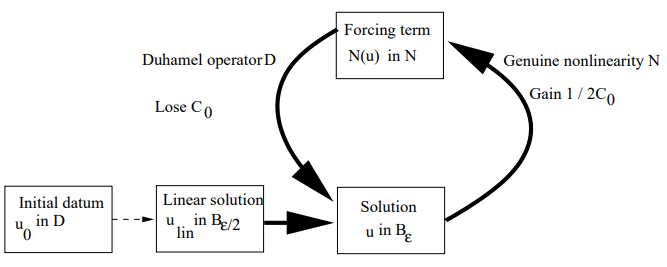
\includegraphics[scale = 0.8]{duhamel}
			\caption{The abstract Duhamel iteration scheme.}
		\end{center}
	\end{figure}

\begin{lemma}[Abstract Duhamel iteration]
	Let $\cN$ and $\cS$ be Banach spaces. Suppose  $D: \cN \to \cS$ is a bounded linear operator such that
		\[ ||DF||_{\cS} \leq C ||F||_{\cN}, \]
	and	 $N : \cS \to \cN$ is a Lipschitz non-linear operator such that $N(0) = 0$ and 
		\[ ||Nu - Nv||_{\cN} \leq \frac{1}{2C} ||u - v||_{\cS}, \]
	for all $u, v \in \overline{B_\epsilon (0)}$. Then for all $u_{\text{lin}} \in \overline{B_{\epsilon/2} (0)}$, there exists a unique solution $u \in \overline{B_\epsilon (0)}$ to the equation (\ref{eq:abs}), with the map $u_{\text{lin}} \mapsto u$ Lipschitz with constant at most $2$.
\end{lemma}

\begin{proof}
	Solving the equation (\ref{eq:abs}) is equivalent to finding a fixed point of the operator $\Phi : \cS \to \cS$ defined by 
		\[ \Phi (u) := u_{\text{lin}} + DNu. \]
	We claim this map is a contraction on the closed ball $\overline{B_\epsilon (0)} \subseteq \cS$ with Lipschitz constant $\tfrac12$; the contraction mapping principle completes the proof. To show $\Phi$ maps the ball into itself, observe by the triangle inequality
		\[ ||\Phi (u)||_\cS \leq ||u_{\text{lin}}||_\cS + ||DNu||_\cS \leq \epsilon \]
	for any $u \in \overline{B_\epsilon (0)}$. To show $\Phi$ is a contraction, for any $u, v \in \cS$, we can write $\Phi(u) - \Phi(v) = D(Nu - Nv)$. Taking norms, we obtain 
		\[ ||\Phi (u) - \Phi(v)||_\cS \leq C ||Nu - Nv||_\cN \leq  \frac12 ||u - v||_\cS,  \]
	as desired. Similarly, to show that the linear-to-nonlinear solution map is Lipschitz continuous, we use the equation and the triangle inequality to write
		\[ ||u - v||_\cS \leq ||u_{\text{lin}} - v_{\text{lin}}||_\cS + ||D(Nu - Nv)||_\cS \leq ||u_{\text{lin}} - v_{\text{lin}}||_\cS + \frac12||u - v||_\cS.  \]
	Rearranging shows that the Lipschitz constant is at most $2$. 	
\end{proof}

\begin{remark}
	One should think of the space $\cS$ as the \textit{solution space} and $\cN$ as the space where the non-linearity resides. Making a judicious choice of these spaces so that the iteration scheme converges is a central problem in the study of semi-linear partial differential equations for small data. 
\end{remark}

\begin{figure}[h]
	\begin{center}
		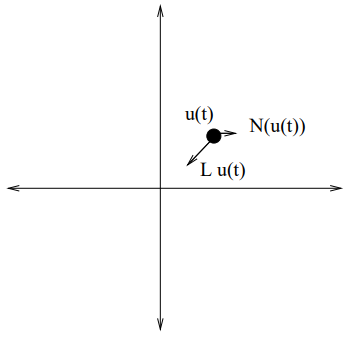
\includegraphics[scale = 0.7]{smalldata}
		\caption{For small data, the dissipative effect of the linear term $Lu$ dominates the non-linear term $Nu$, leading to global well-posedness and decay. }
	\end{center}
\end{figure}

\begin{theorem}[Linear stability implies non-linear stability]
	Let $L \in \operatorname{End} (\R^n)$ be a dissipative linear operator in that 
		\[ \langle Lu, u \rangle \leq - \sigma \langle u, u \rangle\]
	for some $\sigma > 0$, and suppose $N \in C^2_{\loc} (\R^n \to \R^n)$ vanishes faster than linearly at the origin. Then for initial data sufficiently close to the origin $|u_0| \ll 1$, there exists a unique global solution $u \in C^1 ([0, \infty) \to \R^n)$ to the semi-linear equation (\ref{eq:sLin}) obeying the exponential decay,
		\[ |u(t)| \leq 2 e^{-\sigma t} |u_0|. \]
\end{theorem}

\begin{proof}
	Define the solution space $\cS$ and the non-linearity space $\cN$ as subsets of the space of continuous functions $C^0 ([0, \infty) \to \R^n)$ such that the corresponding norms,
		\begin{align*}
			||u||_\cS
				&:= \sup_{t \geq 0} e^{\sigma t} |u(t)|, \\
			||u||_\cN
				&:= \sup_{t \geq 0} e^{\sigma t} |u(t)|
		\end{align*}
	are finite. By Gronwall's inequality, $||u_{\text{lin}}||_\cS \leq |u_0|$, so the triangle inequality implies
		\[ ||DF||_\cS \leq \frac1\sigma ||F||_\cN. \]
	Since $N$ vanishes super-linearly at the origin, Taylor expanding gives $|Nu - Nv| \ll |u - v| (|u| + |v|)$ for all $|u|, |v| \ll 1$. In particular, 
		\[ |N u(t) - Nv(t)| \ll \epsilon e^{-2\sigma t} ||u - v||_\cS. \]
	for $||u||_\cS, ||v||_\cS \leq \epsilon \ll 1$. Rearranging, 
		\[ ||Nu - Nv||_\cN \leq \frac12 \sigma ||u - v||_\cS.  \]
	Applying the abstract Duhamel iteration for $|u_0| \leq \tfrac\epsilon2$ furnishes the desired solution. 	
\end{proof}

\bibliographystyle{alpha}
\bibliography{external/biblio}


\end{document}